\chapter{Implémentation et Validation}
\label{ch:implem}

%\subsection{Implémentation : EA dirigée par les modèles exécutables}
%Implémentation du métamodèle avec Ecore avec EMF et co
%
%Vue intégration : Contrainte OCLinEcore
%Simulation 
%Plugin fUML pour l'exécution de processus métier et la simulation de processus - fUML pour les Smart Grids et pour l'outil papyrus qui permet d'appeler des applications extérieures
%Requête OCLinEcore pour mener l'analyse du comportement
%Transformation de modèles 


\section{Modèles d'architecture d'entreprise pour le cas métier de la gestion d'une flotte de véhicule électrqiue}
Nous éprouvons notre démarche au cas métier de la gestion d'une flotte de véhicules électriques. Nous construisons les modèles adéquats pour les vues métier, fonctionnelle et applicative en adoptant des langages exécutables. La cohérence est modélisée dans la vue intégration. L'architecture globale du cas métier est illustrée dans la \ref{fig:architecture_generale_usecase}.


\begin{figure}[!htbp]
 \begin{center}
  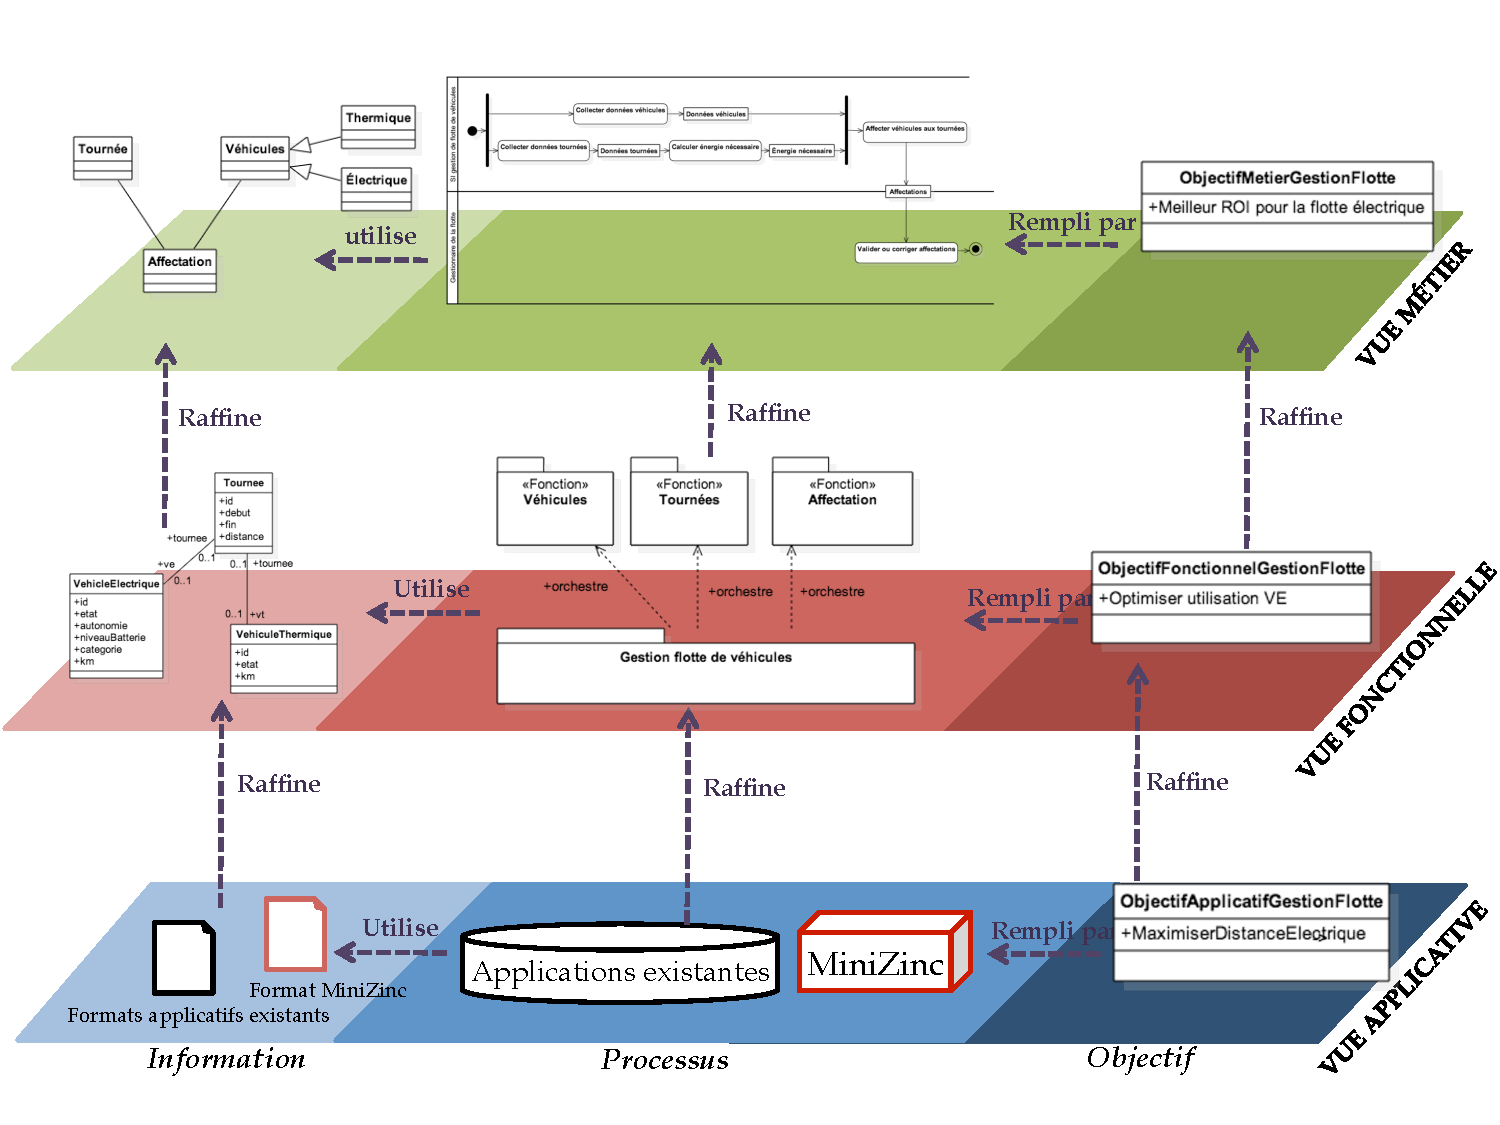
\includegraphics[angle=90, width=1\textwidth]{images/implementation/architecture_generale_usecase.pdf}
 \end{center}
 \caption{Implémentation de l'approche proposé à la gestion de flotte de véhicules}
 \label{fig:architecture_generale_usecase}
\end{figure}


\subsection{Vue métier}
Nous utilisons fUML comme langage exécutable pour modéliser cette vue. Le processus métier consiste à collecter les données relatives aux véhicules (électriques et thermiques) ainsi qu'aux tournées à effectuer, de calculer l'énergie nécessaire à chaque tournée et l'affectation véhicule/tournée avant de faire valider cette dernière par le manager de flotte. Nous modélisons ce processus métier sous forme de diagramme d'activité fUML et le simulons en utilisant Papyrus. Selon notre cadre d'architecture, les modèles créés représentent donc l'aspect processus de la vue métier.

Pour l'aspect information, nous utilisons des diagrammes de classe UML pour représenter les concepts métier et leurs relations. Nous modélisons ainsi les concepts de Véhicule, Tournée et Affectation.
Gérer une flotte de véhicules peut avoir plusieurs objectifs métier. Dans notre cas, obtenir le meilleur retour sur investissement suite à l'intégration de véhicules électriques dans la flotte de véhicules. Nous modélisons l'objectif métier sous la forme d'une classe UML.

Le choix des langages de modélisation et de l'outil de simulation est motivé par les pratiques du domaine. En effet, la Commission Électrique Internationale a adopté Enterprise Architect comme outil pour maintenir et distribuer le CIM\footnote{Common Information Model}\cite{uslar2012standardization}, un modèle d'information commun pour le domaine électrique \footnote{www.sparxsystems.com.au/press/articles/iec.html}.
	

\subsection{Vue fonctionnelle}

Nous modélisons l'aspect information sous la forme d'une diagramme de classe fUML. Ce modèle raffine les concepts métier en spécifiant leurs types. Dans la vue fonctionnelle, le concept d'allocation prend la forme d'une association entre les véhicules et les tournées. L'objectif fonctionnel est modélisé sous la forme d'une classe UML. L'objectif fonctionnel spécifie qu'il faut optimiser l'utilisation des véhicules électriques pour atteindre l'objectif métier qui est d'avoir un meilleur retour sur investissement.

Pour l'aspect processus, nous commençons par identifier trois blocs fonctionnels : un bloc pour la gestion de la flotte de véhicules (électriques et thermiques), un bloc pour la gestion des tournées, un bloc pour la gestion de l'affectation (voir figure \ref{fig:architecture_generale_usecase}. Ces blocs contiennent les fonctions qui raffinent les tâches du processus métier. Comme expliqué plus tôt dans la démarche, le fait de les rassembler dans des blocs selon les concepts métier augmente la modularité et l'évoluvilité de l'architecture. De plus, nous consacrons un bloc à la gestion des processus fonctionnels. Ce bloc est responsable de l'orchestration des fonctions du processus fonctionnel. 

Les blocs fonctionnels offrent une vue plus détaillée des tâches métier. Il est possible de modéliser les différentes fonctions (calcul des tournées à partir de bon de travaux, calcul de l'énergie nécessaire à une tournée, etc.) à l'aide de diagrammes d'activité exécutables. Le choix du langage de modélisation dépend du cas d'application. Par exemple, nous modélisons l'affectation véhicule/tournée sous la forme de contraintes OCL~:~pour affecter un véhicule à une tournée, il faut que l'énergie nécessaire à celle-ci soit inférieure à l'autonomie de la batterie. Dans notre cas d'application, nous considérons qu'il n'est pas possible de recharge le véhicule pendant la tournée de l'agent.

Nous considérons un premier cas où il n'est pas possible de recharger la batterie au cours de la tournée. L'aspect \emph{information} de la vue fonctionnelle prend la forme de données fonctionnelles  modélisées par un diagramme de classes sur lequel s'appliquent les contraintes OCL (\ref{fig:architecture_generale_usecase}). OCL est adapté aux diagrammes de classes. De plus, OCL est un langage standardisé et exécutable pour l'expression de contraintes. Il est possible de modéliser les autres algorithmes de traitement (calcul des tournées à partir de bon de travaux, calcul de l'énergie nécessaire à une tournée, etc.) à l'aide de diagrammes d'activité exécutables.

En utilisant le langage OCL, nous modélisons la fonction d'affectation sous la forme de deux contraintes et d'une requête. La première contrainte OCL signifie que si un véhicule électrique est affecté à une tournée alors l'énergie dont il dispose permet d'assurer la totalité de la tournée.
La deuxième contrainte signifie que si aucun véhicule électrique n'est capable d'assurer une tournée donnée alors c'est un véhicule thermique qui lui est associé. Enfin, la requête calcule le nombre total de kilomètres électriques correspondant à la distance parcourue par les véhicules électrique après l'affectation. Cette requête permet d'évaluer l'utilisation  des véhicules électriques dans l'optique d'atteindre l'objectif fonctionnel.

\begin{queryl}[linewidth=15cm]
context Tournee
inv : 
self.ve.autonomie * self.ve.niveauBatterie > self.energieRequise

context Tournee
inv : self.ve <> undefined xor self.vt <> undefined

context Tournee :: elecKm() : int
body :  
(Tournee::allInstances() -> collect(t.ve <> undefined|t.distance)) 
-> sum()
\end{queryl}


\subsection{Vue applicative}

Pour les processus applicatifs, nous commençons par identifier 
les applications nécessaires à l'implantation des blocs fonctionnels. Dans notre cas, le patrimoine applicatif de l'entreprise dispose déjà d'applications pour la gestion de tournées (calcul de tournées optimisé à partir de bons de travaux) et la gestion de véhicules (administration, maintenance, etc.). Pour la fonction d'allocation, nous faisons le choix d'utiliser MiniZinc pour modéliser les contraintes au niveau applicatif \ref{fig:contraintesMiniZinc}. 

\begin{figure}[!htbp]
 \begin{center}
  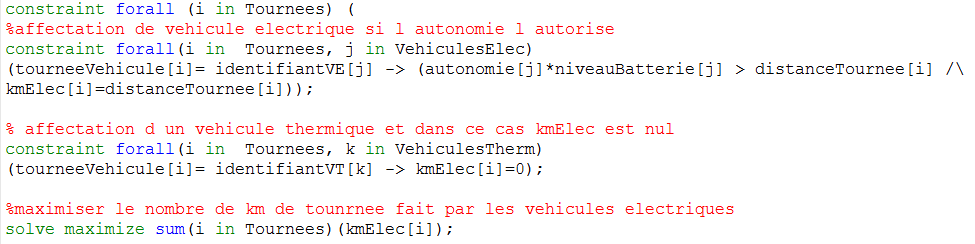
\includegraphics[width=1\textwidth]{images/implementation/module_minizinc.png}
 \end{center}
 \caption{Contraintes du module MiniZinc}
 \label{fig:contraintesMiniZinc}
\end{figure} 

MiniZinc est un langage de modélisation et de résolution de contraintes de niveau intermédiaire qui a pour vocation de devenir un langage de modélisation standard dans le domaine de la programmation par contraintes. L'aspect information contient les formats de données nécessaires aux différentes applications. La figure \ref{fig:formatMiniZinc} représente le fichier de données (le format .dzn) nécessaire à l'application MiniZinc pour calculer l'affectation. 

\begin{figure}[!htbp]
 \begin{center}
  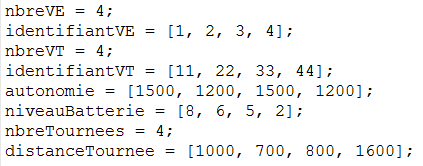
\includegraphics[width=0.5\textwidth]{images/implementation/format_minizinc.png}
 \end{center}
 \caption{Fichier de données pour le module MiniZinc}
 \label{fig:formatMiniZinc}
\end{figure} 

L'objectif applicatif est modélisé sous la forme d'une classe fUML. Un véhicule électrique devient rentable par rapport à un véhicule thermique à partir d'un certain nombre de kilomètre parcouru. C'est pourquoi l'objectif fonctionnel qui est d'optimiser l'usage de la flotte électrique se traduit par la maximisation du nombre de kilomètres électriques, c'est à dire affecter aussi souvent que possible un véhicule électrique aux tournées. Ainsi, le module MiniZinc prend en compte cet objectif en résolvant les contraintes tout en maximisant la distance électrique. 

\subsection{Vue intégration}

Nous modélisons la vue intégration en spécifiant les liens de cohérence  intra-vue et et inter-vues. Les contraintes que ces liens doivent respecter sont spécifiés dans le métamodèle du cadre d'architecture présenté dans la démarche. La figure \ref{fig:integration_gestion_flotte} offre une vue partielle des modèles d'intégration. Nous y modélisons à titre d'illustration les liens de cohérence intravue entre la fonction d'affection, ses inputs et output et son objectifs fonctionnel. Nous faisons de même pour le module d'optimisation Minizinc, ses inputs et outputs ainsi que l'objectif applicatif qu'il remplit. Le même principe d'intégration «~horizontale~», c'est à dire entre les aspects d'une même vue, est appliqué à tous les autres éléments de la vue métier, fonctionnelle et applicative. Nous mettons l'ensemble des modèles de la vue intégration en annexe de ce manuscrit. 

De la même manière, nous modélisons les liens de cohérence inter-vues. Par exemple, le lien «~inputs~» exprime qu'un type de données est compatible avec la fonction qui l'utilise et qu'un format est compatible avec le module applicatif qui l'utilise en entrée. Pour garantir une bonne orchestration des processus, il faut que le «~outputs~» d'une tâche (respectivement une fonction, un module applicatif) soit compatible avec le «~inputs~» de la tâche suivante (respectivement une fonction, un module applicatif).

Les éventuelles transformation de modèles sont aussi identifiées dans la vue intégration. Pour le cas métier de la gestion de flotte de véhicules, nous utilisons une transformation de modèle pour générer les contraintes pour le module de calcul d'affectation MiniZinc de la vue applicative à partir des contraintes OCL exprimées dans la fonction affectation de la vue fonctionnelle. La transformation est écrite dans le langage de transformation Acceleo (Annexe Acceleo). En plus de transformer les contraintes décrite dans l'aspect métier, cette transformation de modèle permet aussi de transformer les instances des types fonctionnels en instances dans le format dzn utilisé par le module MiniZinc comme l'illustre la figure \ref{fig:integration_gestion_flotte}. 

\begin{figure}[!htbp]
 \begin{center}
  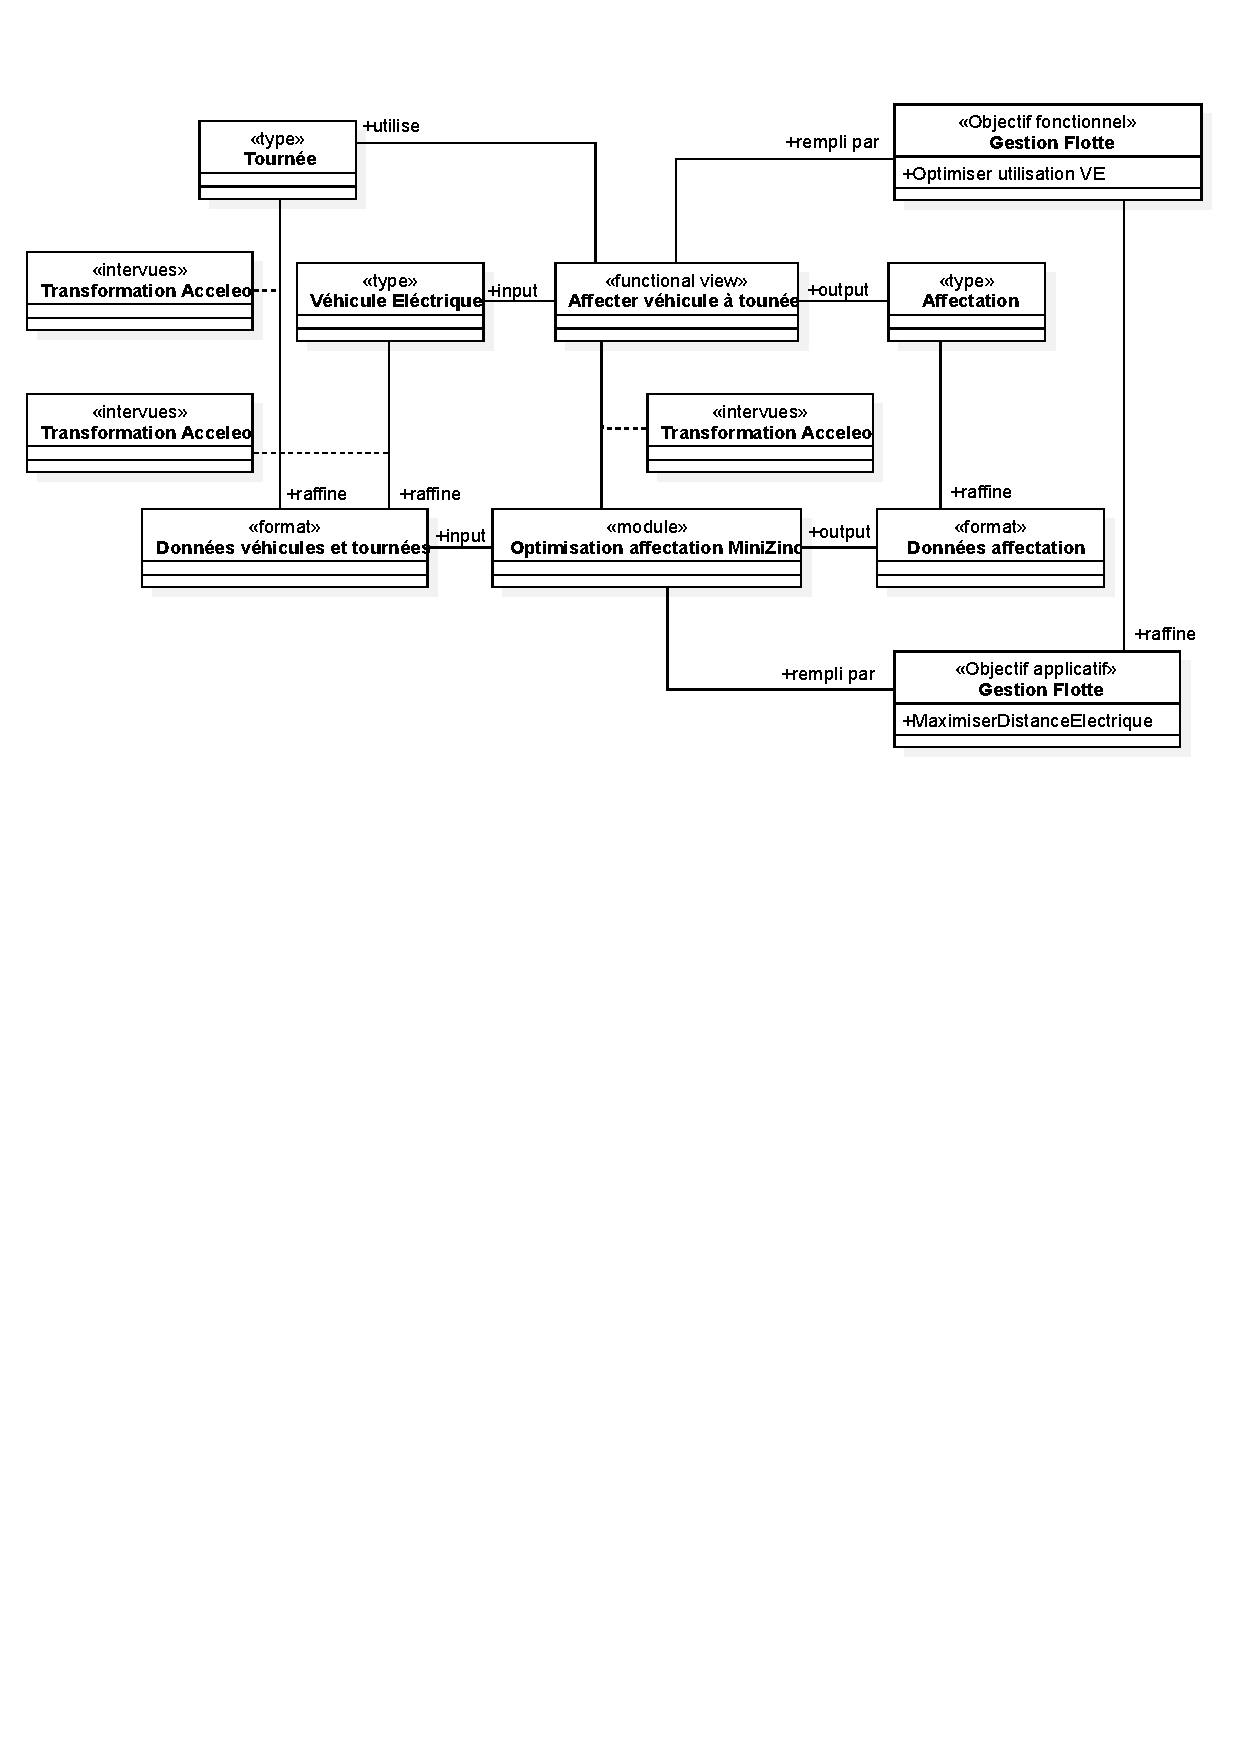
\includegraphics[trim= 0cm 16cm 0cm 0cm, width=1\textwidth]{images/implementation/integration_affection_gestion.pdf}
 \end{center}
 \caption{Une vue partielle des modèles d'intégration de la vue fonctionnelle et de la vue applicative}
 \label{fig:integration_gestion_flotte}
\end{figure}

\section{Analyse par simulation des modèles d'architecture}

Analyse du comportement des modèles d'architecture se fait directement dans les langages de modélisation. Comme nous l'expliquons dans notre démarche, la simulation de l'ensemble de l'architecture est pilotée par l'exécution du processus métier. La simulation du processus métier se traduit par l'exécution du diagramme d'activité fUML. Nous utilisons Papyrus comme outil de modélisation et de simulation du processus métier de gestion de flotte de véhicule. En effet, Papyrus implémente la sémantique d'exécution fUML telle qu'elle est spécifiée par l'OMG. 

Notre démarche préconise de modéliser les détails des taches dans les vues inférieure afin de respecter le niveau d'abstraction requis par chaque point de vue et ainsi de ne pas altérer la compréhension des parties prenantes de la vue qui leur destinée. Par exemple, l'analyse métier n'aura ainsi pas à discuter du détails des applications implémentant les taches métier avec l'architecte applicatif.

Papyrus offre la possibilité d'étendre la sémantique d'exécution de fUML à travers les «~Opaque Actions~». Celles-ci permettent d'invoquer des modules d'applications extérieures au moment de l'exécution du diagramme d'activité fUML. Un stagiaire a développé cette extension en collaboration avec l'équipe Triskel. L'extension permet d'invoquer directement le module MiniZinc pour optimiser l'affectation des véhicules aux tournées.

La simulation prend la forme d'une animation de diagramme. La figure \ref{fig:simu_capture_ecran} est une capture d'écran montrant une simulation en court d'exécution. Papyrus permet aussi de mettre des «~breakpoints~» sur certaines activités et de paramétrer le pas de temps pour contrôler le déroulement du processus.

\begin{figure}[!htbp]
 \begin{center}
  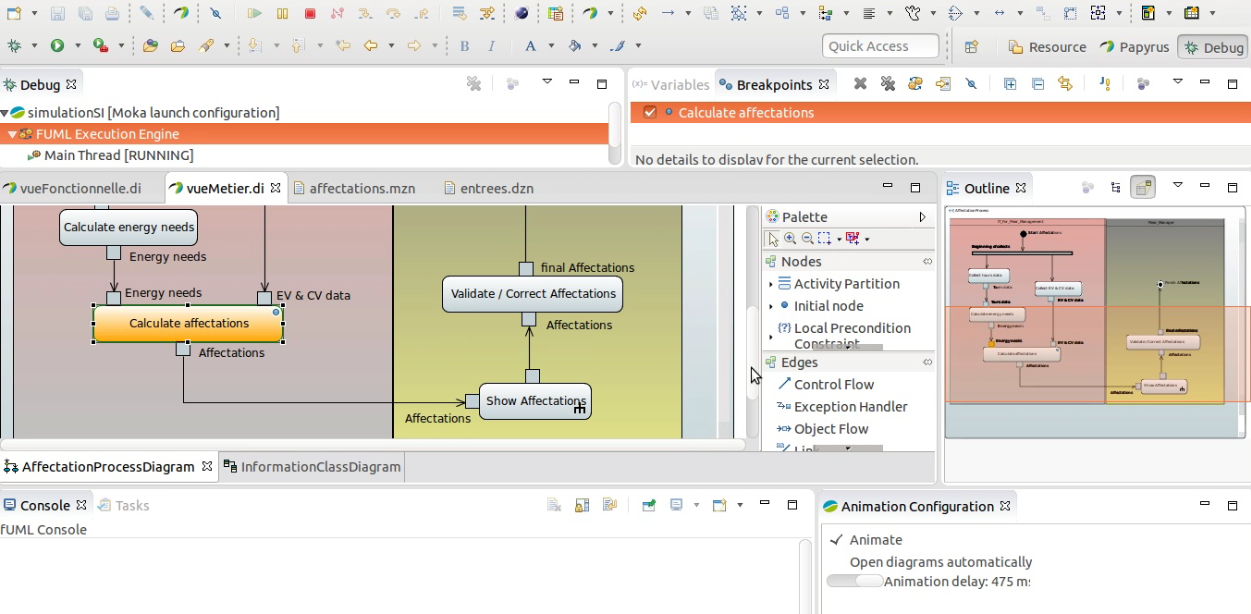
\includegraphics[width=1\textwidth]{images/implementation/simu_capture_ecran.png}
 \end{center}
 \caption{Simulation de l'architecture sous Papyrus}
 \label{fig:simu_capture_ecran}
\end{figure}

La simulation retourne comme résultat les affectations des véhicles aux tournées. Ce résultat est affiché dans la console comme l'illustre la figure \ref{fig:resultat_simu}. La simulation a pour objectif de voir si l'utilisation des véhicules électrique est rentable en comparant la distance parcourue par le véhicule électrique et la distance minimale permettant de le rentabiliser. Dans ce cas, il est par exemple envisageable de reconfigurer les tournées de manière à ce que plus de véhicules électriques soient affectés. En effet, notre démarche a pour but l'analyse fonctionnelle. La validation s'appuie sur les indicateurs dérivés de l'aspect objectif et sur l'avis des experts. Des analyses statistiques peuvent être conduites mais elles ne rentrent pas dans le périmètre de nos travaux.


\begin{figure}[!htbp]
 \begin{center}
  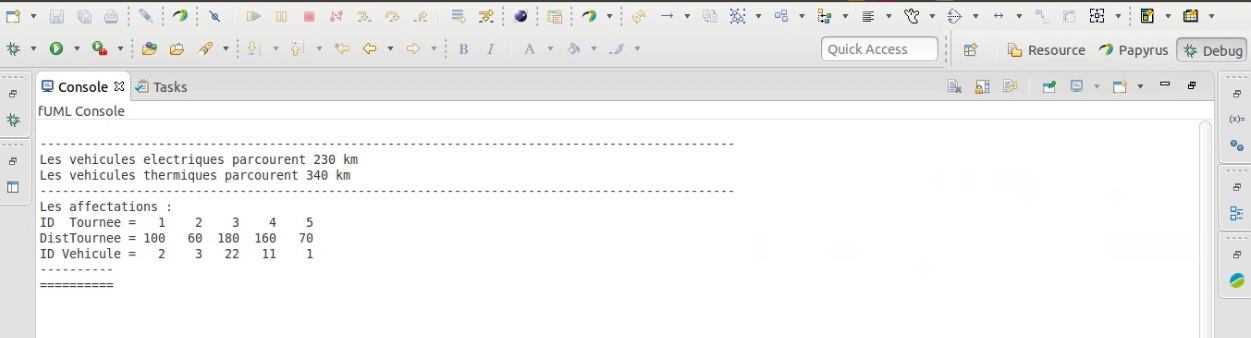
\includegraphics[width=1\textwidth]{images/implementation/resultat_simu.png}
 \end{center}
 \caption{Résultat retournée par la simulation l'architecture sous Papyrus}
 \label{fig:resultat_simu}
\end{figure} 


%\section{analyse de la structure}
%Validate modèle -> pour tester l'intégrité du modèle
%Requêtes sur le modèle OCL
%Si appli hirs service quel sont les processus impacté etc.
%Un nouveau process faisant intervenir d'ancienne tâche, quelle ancienne appli réutilisée
%Détecter les problèmes d'interop' entre modules
 






\lstinputlisting{figures/minizinc/affectations.mzn}

